\subsection*{Pertanyaan 1: Analisis graf berarah pada Gambar 6.4 dan tuliskan urutan jalurnya secara manual apabila menggunakan algoritma BFS dan DFS mulai dari simpul/node ke-0!}

\textbf{Graf Gambar 6.4 (7 simpul):} Edge: 0 $\rightarrow$ 1, 0 $\rightarrow$ 2, 1 $\rightarrow$ 3, 2 $\rightarrow$ 3, 2 $\rightarrow$ 4, 3 $\rightarrow$ 5, 4 $\rightarrow$ 5, 4 $\rightarrow$ 6

\begin{figure}[H]
    \centering
    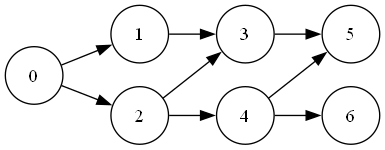
\includegraphics[width=0.65\textwidth]{figures/praktikum6/graf_pretest.png}
    \caption{Visualisasi Graf Pre Test (Gambar 6.4)}
\end{figure}
\vspace{1em}
\textbf{Jawaban BFS manual dari node 0:}
\begin{table}[H]
    \centering
    \caption{Penelusuran BFS Manual dari Node 0}
    \begin{tabular}{lllp{6cm}}
    \toprule
    \textbf{Langkah} & \textbf{Node Diproses} & \textbf{Antrian Setelah} & \textbf{Alasan} \\ \midrule
    1 & 0 & [1, 2] & kunjungi 0, masukkan tetangga 1 dan 2 \\
    2 & 1 & [2, 3] & kunjungi 1, masukkan tetangga 3 \\
    3 & 2 & [3, 4] & kunjungi 2, masukkan 4 (3 sudah di antrian) \\
    4 & 3 & [4, 5] & kunjungi 3, masukkan tetangga 5 \\
    5 & 4 & [5, 6] & kunjungi 4, masukkan 6 (5 sudah di antrian) \\
    6 & 5 & [6] & kunjungi 5, tidak ada tetangga baru \\
    7 & 6 & [] & kunjungi 6, tidak ada tetangga baru \\ \bottomrule
    \end{tabular}
\end{table}
Urutan BFS: 0, 1, 2, 3, 4, 5, 6

\vspace{1em}
\textbf{Jawaban DFS manual dari node 0:}
\begin{table}[H]
    \centering
    \caption{Penelusuran DFS Manual dari Node 0}
    \begin{tabular}{llp{9cm}}
    \toprule
    \textbf{Langkah} & \textbf{Node} & \textbf{Aksi} \\ \midrule
    1 & 0 & kunjungi 0, rekursi ke tetangga pertama: 1 \\
    2 & 1 & kunjungi 1, rekursi ke tetangga: 3 \\
    3 & 3 & kunjungi 3, rekursi ke tetangga: 5 \\
    4 & 5 & kunjungi 5, tidak ada tetangga, backtrack ke 3, ke 1, ke 0 \\
    5 & 2 & dari 0 rekursi ke tetangga berikutnya: 2 \\
    6 & 4 & kunjungi 2, rekursi ke 4 (3 dan 5 sudah dikunjungi) \\
    7 & 6 & kunjungi 4, rekursi ke 6 (5 sudah dikunjungi) \\ \bottomrule
    \end{tabular}
\end{table}
Urutan DFS: 0, 1, 3, 5, 2, 4, 6

\subsection*{Pertanyaan 2: Apa perbedaan utama antara algoritma BFS dan DFS?}

\begin{table}[H]
    \centering
    \caption{Perbedaan Algoritma BFS dan DFS}
    \begin{tabular}{p{3.5cm}p{5cm}p{5cm}}
    \toprule
    \textbf{Aspek} & \textbf{BFS} & \textbf{DFS} \\ \midrule
    Strategi penelusuran & Melebar (level by level) & Mendalam (cabang habis dulu) \\
    Struktur data & Queue (antrian) & Stack / Rekursi \\
    Kompleksitas memori & O(V) untuk antrian & O(H), H = kedalaman rekursi \\
    Jalur terpendek & Menjamin pada graf tidak berbobot & Tidak menjamin \\
    Penggunaan utama & Shortest path, web crawling & Deteksi siklus, topological sort \\
    Kompleksitas waktu & O(V + E) & O(V + E) \\ \bottomrule
    \end{tabular}
\end{table}